%%%% Proceedings format for most of ACM conferences (with the exceptions listed below) and all ICPS volumes.
\documentclass[sigconf]{acmart}
%%%% As of March 2017, [siggraph] is no longer used. Please use sigconf (above) for SIGGRAPH conferences.

%\usepackage[brazilian]{babel}
\usepackage[utf8]{inputenc}
\usepackage[T1]{fontenc}
\usepackage{graphicx}
\usepackage{listings}
\usepackage{amsmath}
\usepackage{csvsimple}
\usepackage{tabularx}
\usepackage{soul}


\lstdefinestyle{mystyle}{
	basicstyle=\scriptsize\ttfamily,
	numberstyle=\tiny\itshape,
	frame=single,
	breakatwhitespace=false,
	breaklines=true,
	captionpos=b,
	keepspaces=true,
	numbers=left,
	xleftmargin=2.6em,
	framexleftmargin=2em,
	showspaces=false,
	showstringspaces=false,
	showtabs=false,
	tabsize=2
}

\lstdefinelanguage{claret} {
	morekeywords={systemName, system, usecase, actor, version, preCondition, postCondition, basic, step, alternative, exception, af, ef, bs, user, type, date},
	sensitive=false,
	morecomment=[l]{//},
	morecomment=[s]{/*}{*/},
	morestring=[b]"
}

%\usepackage{color}
\newcommand{\correct}[1]{#1}

\usepackage{flushend}


%%%% Proceedings format for SIGPLAN conferences 
% \documentclass[sigplan, anonymous, review]{acmart}

%%%% Proceedings format for SIGCHI conferences
% \documentclass[sigchi, review]{acmart}

%%%% To use the SIGCHI extended abstract template, please visit
% https://www.overleaf.com/read/zzzfqvkmrfzn

%
% defining the \BibTeX command - from Oren Patashnik's original BibTeX documentation.
\def\BibTeX{{\rm B\kern-.05em{\sc i\kern-.025em b}\kern-.08emT\kern-.1667em\lower.7ex\hbox{E}\kern-.125emX}}
    
% Rights management information. 
% This information is sent to you when you complete the rights form.
% These commands have SAMPLE values in them; it is your responsibility as an author to replace
% the commands and values with those provided to you when you complete the rights form.
%


% These commands are for a PROCEEDINGS abstract or paper.
\copyrightyear{2019}
\acmYear{2019}
\acmConference[SBES 2019]{XXXIII Brazilian Symposium on Software Engineering}{September 23--27, 2019}{Salvador, Brazil}
\acmBooktitle{XXXIII Brazilian Symposium on Software Engineering (SBES 2019), September 23--27, 2019, Salvador, Brazil}
\acmPrice{15.00}
\acmDOI{10.1145/3350768.3350790}
\acmISBN{978-1-4503-7651-8/19/09}

%
% These commands are for a JOURNAL article.
%\setcopyright{acmcopyright}
%\acmJournal{TOG}
%\acmYear{2018}\acmVolume{37}\acmNumber{4}\acmArticle{111}\acmMonth{8}
%\acmDOI{10.1145/1122445.1122456}

%
% Submission ID. 
% Use this when submitting an article to a sponsored event. You'll receive a unique submission ID from the organizers
% of the event, and this ID should be used as the parameter to this command.
%\acmSubmissionID{123-A56-BU3}

%
% The majority of ACM publications use numbered citations and references. If you are preparing content for an event
% sponsored by ACM SIGGRAPH, you must use the "author year" style of citations and references. Uncommenting
% the next command will enable that style.
%\citestyle{acmauthoryear}

%
% end of the preamble, start of the body of the document source.
\begin{document}

%
% The "title" command has an optional parameter, allowing the author to define a "short title" to be used in page headers.
%
% The "author" command and its associated commands are used to define the authors and their affiliations.
% Of note is the shared affiliation of the first two authors, and the "authornote" and "authornotemark" commands
% used to denote shared contribution to the research.

\title{Reducing the Discard of MBT Test Cases using Distance Functions}
%\title{Using Distance Functions to Classify the Impact of Use Case Edits and Reduce the Discard of MBT Test Cases}

\author{Thomaz Diniz}
\email{thomaz.morais@ccc.ufcg.edu.br}
\affiliation{
  \institution{Federal University of Campina Grande}
  %\streetaddress{R. Aprígio Veloso, 882 - Universitário}
%   \city{Campina Grande}
%   \state{Paraíba}
%   \postcode{58429-900}
}
\author{Everton L.G. Alves}
\email{everton@computacao.ufcg.edu.br}
\affiliation{
  \institution{Federal University of Campina Grande}
%   \streetaddress{R. Aprígio Veloso, 882 - Universitário}
%   \city{Campina Grande}
%   \state{Paraíba}
%   \postcode{58429-900}
}

\author{Anderson G.F. Silva}
\email{andersongfs@splab.ufcg.edu.br}
\affiliation{
  \institution{Federal University of Campina Grande}
%   \streetaddress{R. Aprígio Veloso, 882 - Universitário}
%   \city{Campina Grande}
%   \state{Paraíba}
%   \postcode{58429-900}
}

\author{Wilkerson L. Andrade}
\email{wilkerson@computacao.ufcg.edu.br}
\affiliation{
  \institution{Federal University of Campina Grande}
%   \streetaddress{R. Aprígio Veloso, 882 - Universitário}
%   \city{Campina Grande}
%   \state{Paraíba}
%   \postcode{58429-900}
}


%
% By default, the full list of authors will be used in the page headers. Often, this list is too long, and will overlap
% other information printed in the page headers. This command allows the author to define a more concise list
% of authors' names for this purpose.
%\renewcommand{\shortauthors}{Thomaz, et al.}

%
% The abstract is a short summary of the work to be presented in the article.
\begin{abstract}
%During software evolution test suites are often used as safety net for avoiding feature regression. 
Model-Based Testing (MBT) is used for generating test suites from system models. However, as software evolves, its models tend to be updated, which often leads to obsolete test cases that are discarded. Test case discard can be very costly since essential data, such as execution history, are lost. In this paper, we investigate the use of distance functions to help to reduce the discard of MBT tests. For that, we ran a series of empirical studies using artifacts from industrial systems, and we analyzed how ten distance functions can classify the impact of MBT-centred use case edits. Our results showed that distance functions are effective for identifying low impact edits that lead to test cases that can be updated with little effort. Moreover, we found the optimal configuration for each distance function. Finally, we ran a case study that showed that, by using distance functions, we could reduce the discard of test cases by 15\%.  
\end{abstract}

%
% The code below is generated by the tool at http://dl.acm.org/ccs.cfm.
% Please copy and paste the code instead of the example below.
%
\begin{CCSXML}
<ccs2012>
<concept>
<concept_id>10011007.10011074.10011099</concept_id>
<concept_desc>Software and its engineering~Software verification and validation</concept_desc>
<concept_significance>500</concept_significance>
</concept>
</ccs2012>
\end{CCSXML}

\ccsdesc[500]{Software and its engineering~Software verification and validation}

\keywords{MBT, distance functions, test suite evolution, agile development}

\maketitle
\section{Introduction}
Software testing plays an important role since it helps gain confidence the software works as expected \citep{Pressman:2007}. Moreover, testing is fundamental for reducing risks and assessing software quality \citep{Pressman:2007}. On the other hand, testing activities are known to be complex and costly. Studies found that nearly 50\% of a project's budget is related to testing \citep{kumar2016impacts}. 

In practice, a test suite can combine manually and automatically executed test cases \citep{manualtesting:2009:Itkonen}. Although automation is always desired, manually executed test cases are still very important. \citet{manualtesting:2009:Itkonen} state that manual testing still plays an important role in the software industry and cannot be fully replaced by automatic testing. For instance, a tester that runs manual tests tends to better exercise a GUI and find new faults. On the other hand, manual testing is often costly \citep{harrold2000testing}.

To reduce the costs related to testing, Model-Based Testing (MBT) can be used. It is a strategy where test suites are automatically generated from specification models (e.g., use cases, UML diagrams) \citep{dalal:mbt:1999,Utting:2006:PMT:1200168}. By using MBT, sound tests can be extracted before any coding, and without much effort.


In agile projects, requirements are often volatile \citep{beck2000extremeprogramming,sutherland2014scrum}. In this scenario, test suites are used as safety nets for avoiding feature regression. Discussions on the importance of test case reuse are not new \citep{von1994domain}. In software engineering, software reuse is key for reducing development costs and improving quality. This is also valid for testing \citep{frakes1994systematic}. A test case that finds faults can be a valuable investment \citep{myers2011art}. Good test cases should be stored as a reusable resource to be used in the future \citep{cai2009test}. In this context, an always updated test suite is mandatory. A recent work proposed lightweight specification artifacts for enabling the use of MBT in agile projects \citep{dalton2018mbtagile}, CLARET. With CLARET, one can both specify requirements using use cases and generate MBT suites from them.


However, a different problem has emerged. As the software evolves (e.g., bug fixes, change requirements, refactorings), both its models and test suite need revisions. Since MBT test suites are generated from requirement models, in practice, as requirements change, the requirement artifacts are updated, new test suites are generated, and the newer suites replace the old ones. Therefore, test cases that were impacted by the edits, instead of updated, are often considered obsolete and discarded \citep{de2016full}. 


Although one may find it easy to generate new suites, regression testing is based on a stable test suite that evolves. Test case discarding implies important historical data that are lost (e.g., execution time, the link faults-to-tests, fault-discovering time). Test case historical data is an important tool for assessing system weaknesses and better manage it, therefore, one should not neglect it. For instance, most defect prediction models are based on historical data \citep{he2012investigation}. Moreover, for some strategies that optimize testing resources allocation, historical data is key \citep{noor2015similarity,anderson2014improving}. By discarding test cases, and their historical data, a project may miss important information for both improving a project and guiding its future actions. Moreover, in a scenario where previously detected faults guide development, missing tests can be a huge loss. Finally, test case discard and poor testing are known as signs of bad management and eventually lead to software development
waste \citep{sedano2017software}.


However, part of a test suite may turn obsolete due to little impacted model updates. Thus, those test cases could be easily reused with little effort and consequently reducing testing discards. Nevertheless, manual analysis is tedious, costly, and time-consuming, which often prevents its applicability in the agile context. In this sense, there is a need for an automatic way of detecting reusable and, in fact, obsolete test cases. 

%Silva et al. \cite{Silva:2018:SIM:3266003.3266009} ran a study with MBT test suites which found that 86\% of the test cases turn obsolete between two consecutive versions of a requirement file, and therefore are discarded. An obsolete test case is a test that includes at least one step that differs from the updated version of the specification document. 

Distance functions map a pair of strings to a number that indicates the similarity level between the two versions \citep{cohen2003distance}. In a scenario where manual test cases evolve due to requirement changes, distance functions can be an interesting tool to help us classify the impact of the changes into a test case.

In this paper, first, we assess and discuss the practical problem of model evolution in MBT suites. To cope with this problem, we propose and evaluate two strategies for automatically classifying model edits and tests aiming at avoiding unnecessary test discards. The first is based on distance functions, while the second combines machine learning and distance values.

This work is an extension over our previous one \citep{diniz2019reducing} including the following contributions:
\begin{itemize}
\item An study using historical data from real industrial projects that investigates the impact of model evolution in MBT suites. We found that 86\% of the test cases turn obsolete between two consecutive versions of a requirement file, and those tests are often discarded. Moreover, 52\% of the found obsolete tests
were caused by \textit{low impact} syntactic edits and could become fully updated with the revision of 25\% of the steps.
\item An automatic strategy based on distance functions for reclassifying reusable test cases from the obsolete set. 
%Empirical studies with industrial data found
% This strategy was evaluated with a series of empirical studies that measured its efficiency using industrial data. We found that all distance functions perform well on classifying \textit{low impacted }model edits  (precision above 94\%). Moreover, we found the optimal configuration for using each function. Finally, 
This strategy was able to reduce test case discard by  9.53\%.
\item An automatic strategy based on machine learning and distance functions %results
for classifying test cases and model change impact. This strategy can classify the impact of edits in use case documents with accuracy above 80\%, it was able to reduce the discard of test cases by 10.4\%, and to identify test cases that should, in fact, be discarded.
\end{itemize}


%We mined the evolution of two projects that use MBT suites, and we use ten distance functions to classify edits between \textit{low impact} (e.g., rewording, typo fixing) --require little test case updating-- and \textit{high impact} (specification and functionality changes) --require much test updating. Our results have found that all ten functions perform well on classifying edit impact. Moreover, we found the optimal configuration for using each function. Finally, we ran a case study in which our strategy was able to reduce the test case discard by at least 15\%.

This paper is organized as follows. In Section \ref{sec:motiv}, we present a motivational example. The needed background is discussed in Section \ref{sec:background}. Section \ref{sec:emp} presents an empirical investigation for assessing the challenges of managing MBT suite during software evolution. Sections \ref{sec:es} and \ref{sec:case} present the strategy for classifying model edits using distance functions and the performed evaluation, respectively. Section \ref{sec:ml} introduces the strategy that combines machine learning and distance values. Section \ref{sec:gd} presents a discussion comparing results from both strategies. In Section \ref{sec:threats}, some threats to validity are cleared. Finally, Sections \ref{sec:related} and \ref{sec:conclud} present related works and the concluding remarks.

\section{Motivational Example} \label{sec:motiv}
Suppose that Ann works in a project and wants to benefit from MBT suites. Her project follows an agile methodology where requirements updates are expected to be frequent. Therefore, she decides to use CLARET \citep{dalton2018mbtagile}, an approach for specifying requirements and generating test suites. 

The following requirement was specified using CLARET's DSL (Listing 1): ``{\it In order to access her email inbox, the user must be registered in the system and provide a correct username and password. In case of an incorrect username or password, the system must display an error message and ask for new data.}''. In CLARET, an \textit{\textbf{ef [flow \#]}} mark refers to a possible exception flow, and a \textbf{\textit{bs [step \#]}} mark indicates a returning point from an exception/alternative to the use case's basic flow.

 \lstset{style=mystyle, language=claret}  \begin{lstlisting}[float=b,caption=Use Case specification using CLARET.]
systemName "Email"
usecase "Log in User" {
    actor emailUser "Email User"
    preCondition "There is an active network connection"
    basic {
        step 1 emailUser "launches the login screen"
        step 2 system "presents a form with username and password fields and a submit button"
        step 3 emailUser "fills out the fields and click on the submit button"
        step 4 system "displays a message" ef[1,2]
    }
    exception 1 "User does not exist in database" {
        step 1 system "alerts that user does not exist"  bs 3
    }
    exception 2 "Incorrect password" {
        step 1 system "alerts that the password is incorrect" bs 3
    }
    postCondition "User successfully logged"
}
\end{lstlisting} \label{specExample}

From this specification, the following test suite can be generated: S1 = \{tc1, tc2, tc3\}, where tc1 = [bs:1 $\rightarrow$ bs:2 $\rightarrow$ bs:3 $\rightarrow$ bs:4], tc2 = [bs:1 $\rightarrow$ bs:2 $\rightarrow$ bs:3 $\rightarrow$ ef[1]:1 $\rightarrow$ bs:3 $\rightarrow$ bs:4], and tc3 = [bs:1 $\rightarrow$ bs:2 $\rightarrow$ bs:3 $\rightarrow$ ef[2]:1 $\rightarrow$ bs:3 $\rightarrow$ bs:4] .

Suppose that in the following development cycle, the use case (Listing 1) was revisited and updated due to both requirement changes and for improving readability. Three edits were performed: (i) the message in line 9 was updated to ``displays a successful message''; (ii) system message in line 12 was updated to ``alerts that username does not exist''; and (iii) both description and system message in exception 3 (line 14) were updated to ``Incorrect username/password combination'' and ``alerts that username and/or password are incorrect'', respectively. 

Since steps from all execution flows were edited (basic, exception 1, and exception 2), Ann 
%decides to, instead of first analyzing the impact of the changes in S1, 
discards S1 and generates a whole new suite. However, part of S1's tests was not much impacted and could be turned to reused with little or no update. For instance, only edit (iii), in fact, changed the semantic of the use case, while (i) and (ii) are updates that do not interfere with the system's behavior. Therefore, only test cases that exercise the steps changed by (iii) should be in fact discarded (tc3). Moreover, test cases that exercise steps changed by (i) and/or (ii) could be easily reused and/or updated (tc1 and tc2). 

We believe that an effective and automatic analyzer would help Ann to decide when to reuse or discard test cases, and therefore reduce the burden of losing important testing data. 

\section{Background}
\label{sec:background}
This section presents the MBT process, the CLARET notation, and the basic idea behind the two strategies used for reducing test case discard, distance functions, and machine learning.

\subsection{Model-Based Testing}
MBT aims to automatically generate and manage test suites from software specification models. MBT may use different model formats to perform its goals (e.g., Labeled Transition System (LTS) \citep{tretmans2008model}, UML diagrams \citep{bouquet2007subset}). As MBT test suites are derived from specification artifacts, their test cases tend to reflect the system behavior \citep{STVR:STVR456}. \citet{Utting:2006:PMT:1200168} discuss a series of benefits of using MBT, such as sound test cases, high fault detection rates, and test cost reduction. On the other hand, regarding MBT limitations, we can list the need for well-built models, huge test suites, and a great number of obsolete test cases during software evolution. 

Figure \ref{fig: mbt_flow} presents an overview of the MBT process. The system models are specified through a DSL (e.g., UML) and a test generation tool is used to create the test suite. However, as the system evolves, edits must be performed on its models to keep them up-to-date.  If any fault is found, the flow goes back to system development. These activities are repeated until the system is mature for release. Note that previous test suites are discarded, and important historical data may be lost in this process.

%On the left-hand side we can see the first test suite generation. However, as the system evolves, edits must be performed on its models to keep them up-to-date (right-hand side). Thus, a new test suite is generated, imported to a test management tool, and run. If any fault is found, the flow goes back to system development. These activities are repeated until the system is mature for release. Note that previous test suites are discarded and important historical data may be lost in this process.

\begin{figure}[h]
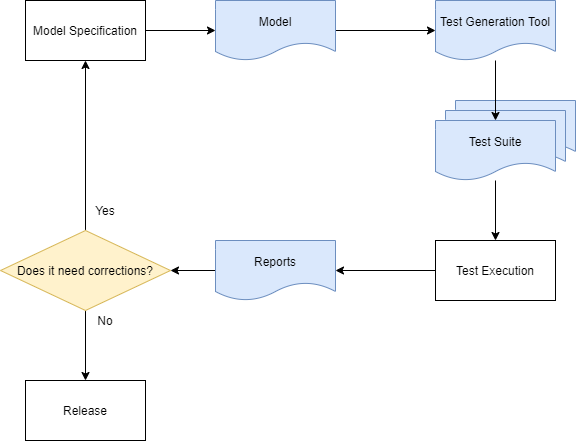
\includegraphics[width=.48\textwidth]{LaTeX/figs/MBT_FLOW_NEW.png}
\caption{MBT Process}
\label{fig: mbt_flow}
\end{figure}


\subsection{CLARET}
CLARET \citep{dalton2017claret,dalton2018mbtagile} is a DSL and tool that allows the creation of use case specifications using natural language. It was designed to be the central artifact for both requirement engineering and MBT practices in agile projects. Its toolset works as a syntax checker for use cases description files and provides visualization mechanisms for use case revision. Listing 1 presents a use case specification using CLARET.  

From the use case description in Listing 1, CLARET generates its equivalent Annotated Labeled Transition System (ALTS) model \citep{tretmans2008model} (Figure \ref{fig:alts}). Transition labels starting with \textit{[c]} indicate pre or post conditions, while the ones starting with \textit{[s]} and \textit{[e]} are regular and exception execution steps, respectively.

\begin{figure}[h!] 
\centering 
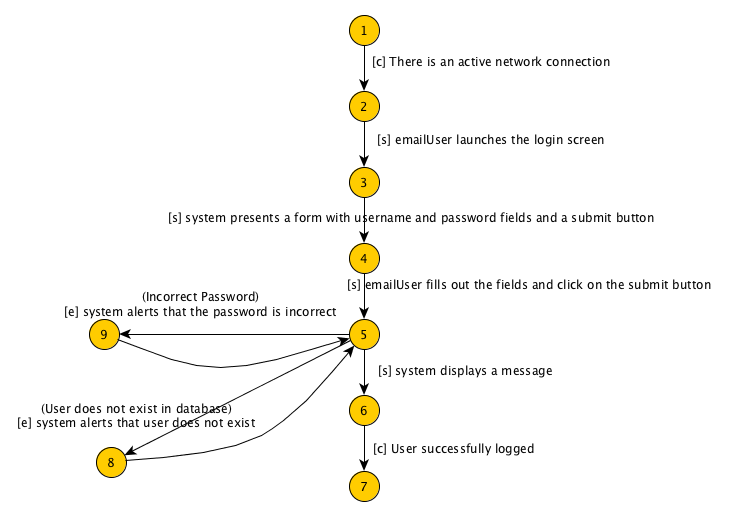
\includegraphics[width=.5\textwidth]{figs/UserLogin.png}
\caption{ALTS model of the use case from Listing 1.}
\label{fig:alts}
\end{figure}

CLARET's toolset includes a test generation tool, LTS-BT (Labeled Transition System-Based Testing) \citep{cartaxo2008lts}. LTS-BT is an MBT tool that uses as input LTS models and generates test suites by searching for valid graph paths. The generated tests are reported in XML files that can be directly imported to a test management tool, TestLink\footnote{http://testlink.org/}.
%Besides generation, it includes a series of algorithms for model-based test selection, reduction, and prioritization. 
The test cases reported in Section \ref{sec:motiv} were collected from LTS-BT.

\subsection{Distance Functions}

Distance functions are metrics for evaluating how similar, or different, are two strings \citep{coutinho2016analysis}. Distance functions have been used in different contexts (e.g., \citep{runkler2000automatic,okuda1976method,lubis2018combination}). For instance, \citet{coutinho2016analysis} use distance functions for reducing MBT suites. 

There are several distance functions (e.g., \citep{hamming1950error,han2007efficient:LCS,huang2008similaritycosine,de1mahalanobis:jaro,Levenshtein_SPD66}). For instance, the Levenshtein function \citep{Levenshtein_SPD66,kruskal1983overview} (equation described below) compares two strings (\textit{a} and \textit{b}) and calculates the number of required operations to transform \textit{a} into \textit{b}, and vice-versa; where $1_{ai \neq bj}$ is the indicator function equal to 0 when $a_{i} \neq b_{j}$ and equal to 1 otherwise, and $lev_{a,b}$ is the distance between the first $i$ characters of \textit{a} and the first $j$ characters of \textit{b}.

To illustrate its use, consider two strings \textit{a} = ``kitten'' and \textit{b} = ``sitting''. Their Levenshtein distance is three, since three operations are needed to transform a to b: (i) replacing `k' by `s'; (ii) replacing `e' by `i'; and (iii) inserting `g' at the end. A more detailed discussion about the Levenshtein and others functions, as well as an open-source implementation of them are available\footnote{https://github.com/luozhouyang/python-string-similarity}.


\resizebox{\columnwidth}{!}{
\begin{equation*}
   lev_{a,b}(i,j) = 
    \begin{cases}
    max(i,j)  \qquad \qquad \qquad \qquad \qquad \text{\textit{if min(i,j) = 0}}&\\
        min 
        \begin{cases}
            lev_{a,b}(i-1,j) + 1\\
            lev_{a,b}(i,j-1) + 1 & otherwise\\ 
            lev_{a,b}(i-1,j-1) + 1_{ai \neq bj} 
        \end{cases}
    \end{cases}
\end{equation*} 
}

\subsection{Machine Learning}

Machine Learning is a branch of Artificial Intelligence based on the idea that systems can learn from data, identify patterns, and make decisions with minimal human intervention \citep{michie1994machine}. By providing ways for building data-driven models, machine learning can produce accurate results and analysis \citep{zhang2003machine}.

The learning process begins with observations or data (examples), it looks for data patterns, and make future decisions. By applying machine learning, one aims to allow computers to learn without human intervention, and to adjust its actions accordingly.

Machine learning algorithms are often categorized as supervised or unsupervised. Supervised machine learning algorithms (e.g., linear regression, logistic regression, neural networks) use labeled examples from the past to predict future events. Unsupervised machine learning algorithms (e.g., k-Means clustering, Gaussian mixture models) are used when the training data is neither classified nor labeled. It infers a function to describe a hidden structure from unlabeled data. 

The use of machine learning in software engineering has grown in the past years. For instance, machine learning methods have been used for estimating development effort \citep{srinivasan1995machine,baskeles2007software}, predicting a software fault-proneness \citep{gondra2008applying}, fault prediction \citep{shepperd2014researcher}, and improving code quality \citep{malhotra2012fault}.

\section{Empirical Study}\label{sec:es}
The study described in Section \ref{sec:emp} evidences the challenge of managing MBT suites during software evolution. To test whether distance functions can help to cope with this problem, we ran a second empirical study. The goal of this study was to analyze the use of distance functions to automatically classify changes in use case documents that could impact MBT suites. 

\subsection{Subjects and Functions}
For that, our study was also run in the context of the industrial projects SAFF and BZC. 
%that were developed in the context of a cooperation between
%our research lab and two different companies, Ingenico do Brasil Ltda and Viceri Solution Ltda. The SAFF project is an information
%system that manages reports on payment terminals,
%and BZC is a system for optimizing e-commerce logistic activities. 
It is important to remember that both projects used agile methodologies to guide the development and updates in the requirement artifacts were frequent. Moreover, their teams used both CLARET \citep{dalton2017claret}, for use case specification, and LTS-BT \citep{cartaxo2008lts} for generating MBT suites. 

%Both projects use manually executed system-level black-box test cases for regression purposes. In this sense, test case history data is very important since can help to keep track of the system evolution and to avoid functionality regression. However, the teams reported that often discard test cases when the related steps on the system use cases are updated in any form, which they refer to as a practical management problem.

As our study focuses on the use of distance functions, we selected a set of ten of the most well-known functions that have been used in different contexts: Hamming \citep{hamming1950error}, LCS \citep{han2007efficient:LCS}, Cosine \citep{huang2008similaritycosine}, Jaro \citep{de1mahalanobis:jaro}, Jaro-Winkler \citep{de1mahalanobis:jaro}, Jaccard \citep{Lu2013SimilaridadeJaccard}, Ngram \citep{Kondrak2005ngram}, Levenshtein \citep{Levenshtein_SPD66}, OSA \citep{Damerau:1964}, and Sorensen Dice \citep{sorensen1948method}. To perform systematic analyses, we normalize their results in a way that their values range from zero to one. Values near zero refer to low similarity, while near one values indicate high similarity. We reused open-source implementations of all ten functions\footnote{https://github.com/luozhouyang/python-string-similarity}\footnote{https://rosettacode.org/wiki/Category:Programming\_Tasks}. To customize and analyze the edits in the context of our study, we created our own tool and scripts that were verified through a series of tests.

%that is available on our website\footnote{Not presented due to double-blind review.}.

We mined the projects' repository and collected all use case edits. Each of these edits would then impact the test cases. We call ``impacted'' any test case that includes steps that were updated during model maintenance. However, we aim to use distance functions to help us to classify these edits and avoid the test case discard.

%\subsection{Research Questions}
To guide our investigation, we defined the following research questions:
\begin{itemize}
\item \textbf{RQ4}: Can distance functions be used to classify the impact of edits in use case documents?  
\item \textbf{RQ5}: Which distance function presents the best results for classifying edits in use case documents?
\end{itemize}

\subsection{Study Setup and Procedure} \label{sec:procedure}
Since all use case documents were CLARET files, we reused the data collected in the study of Section \ref{sec:emp}. Therefore, a total of 79 pairs of use case versions were analyzed in this study, with a total of 518 edits. Table \ref{tab:useCases} summarizes the data.

%mined the projects' repositories and collected, for each file \textit{f}, its history of edits in a time frame. We consider an use case edit any update performed between two consecutive versions (\textit{v1} and \textit{v2}) of \textit{f}. 

% \begin{table}[]
% \centering
% \caption{Summary of the artifacts used in our study.}
% \label{tab:useCases}
% \begin{tabular}{|l|l|l|l|}
% \hline
%      & \#Use Cases & \#Versions &\#Edits \\ \hline
% SAFF &     13      &      42    &     415         \\ \hline
% BZC  &      15     &      37    &     103        \\ \hline
% Total  &      28     &      79    &     518         \\ \hline
% \end{tabular}
% \end{table}

After that, we manually analyzed each edit and classified them between \textit{low impact} and \textit{high impact}. A \textbf{low impact} edit refers to changes that do not alter the system behavior (a pure synthetic edit), while a \textbf{high impact} edit refers to changes in the system expected behavior (semantic edit). Table \ref{tab:class} exemplifies this classification. While the edit in the first line changes the semantics of the original requirement, the next two refer to edits performed for improving readability and fixing typos. During our classification, we found 399 \textit{low impact} and 27 \textit{high impact} edits for the SAFF system, and 92 \textit{low} and 11 \textit{high impact} for BZC. This result shows that use cases often evolve for basic description improvements, which may not justify the great number of discarded test cases in MBT suites.

\begin{table}[]
\caption{Classification of edits.}
\resizebox{\columnwidth}{!}{%
\begin{tabular}{|l|l|l}
\cline{1-2}
\multicolumn{2}{|c|}{\textbf{Steps Description}}                                                                                                                                  &                                              \\ \hline
\multicolumn{1}{|c|}{\textbf{Version 1}}                                       & \multicolumn{1}{c|}{\textbf{Version 2}}                                                 & \multicolumn{1}{c|}{\textbf{Classification}} \\ \hline
\begin{tabular}[c]{@{}l@{}}“Extract data on \\ offline mode.”\end{tabular}     & \begin{tabular}[c]{@{}l@{}}“Show page that \\ requires new data.”\end{tabular}          & \multicolumn{1}{l|}{high impact}             \\ \hline
\begin{tabular}[c]{@{}l@{}}“Show page that \\ requires new data.”\end{tabular} & \begin{tabular}[c]{@{}l@{}}“Show page that \\ requires new terminal\\ data.”\end{tabular} & \multicolumn{1}{l|}{low impact}              \\ \hline
\begin{tabular}[c]{@{}l@{}}"Click on Edit \\ button"\end{tabular}              & \begin{tabular}[c]{@{}l@{}}"Click on the Edit \\ button"\end{tabular}                   & \multicolumn{1}{l|}{low impact}              \\ \hline
\end{tabular}
}
\label{tab:class}
\end{table}

After that, for each edit (original and edited versions), we ran the distance functions using different configuration values and observed how they classified the edits compared to our manual validation. 
%Figure \ref{fig:overview} presents an overview of our study's procedure for a single project.

% \begin{figure}[h]
% \centering
% 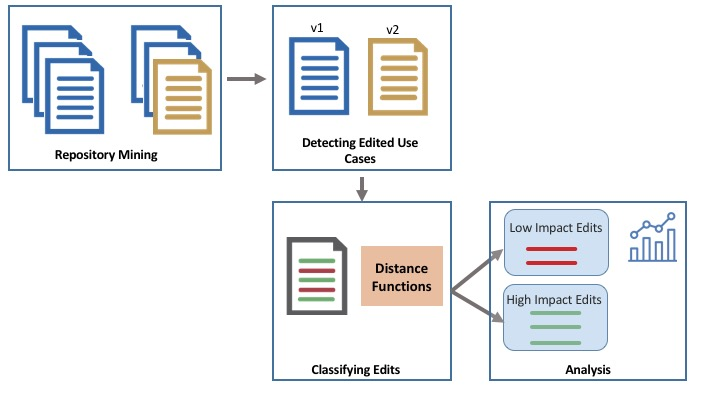
\includegraphics[height=2.3in,width=3.3in]{figs/overview.jpg}
% \caption{Study overview for a single subject.}
% \label{fig:overview}
% \end{figure}

\subsection{Metrics}

To help us evaluate the results, and answer our research questions, we used three of the most well-known metrics for checking binary classifications: \textit{Precision}, which is the rate of relevant instances among the found ones; \textit{Recall}, calculates the rate of relevant retrieved instances over the total of relevant instances; and \textit{Accuracy}, which combines Precision and Recall. These metrics have been used in several software engineering empirical studies (e.g., \citep{nagappan2008influence,hayes2005text, elish2008predicting}). Equations \ref{eq:precision}, \ref{eq:recall} and \ref{eq:acc} present those metrics, where TP refers to the number of cases a distance function classified an edit as low impact and the manual classification confirms it; TN refers to the number of matches regarding high impact edits; FP refers to when the automatic classification reports low impact edits when in fact high impact edits were found; and FN is when the automatic classification reports high impact when in fact should be low impact edits.   

\begin{equation} \label{eq:precision}
Precision = \frac{TP}{TP+FP}
\end{equation}

\begin{equation} \label{eq:recall}
Recall = \frac{TP}{TP+FN}
\end{equation}

\begin{equation} \label{eq:acc}
Accuracy = \frac{TP+TN}{TP+TN+FP+FN}
\end{equation}


\subsection{Results and Discussion} \label{sec:res}

To answer RQ4, we first divided our dataset of use case edits into two (low and high impact edits), according to our manual classification. Then, we ran the distance functions and plotted their results. Figures \ref{fig:bp_dist_l} and \ref{fig:bp_dist_h} show the box-plot visualization of this analysis considering found low (Figure \ref{fig:bp_dist_l}) and high impacts (Figure \ref{fig:bp_dist_h}). As we can see, most low impact edits, in fact, refer to low distance values (median lower than 0.1), for all distance functions. This result gives us evidence that low distance values can relate to low impact edits and, therefore, can be used for predicting low impact changes in MBT suites. On the other hand, we could not find a strong relationship between high impact edits and distance values. Therefore we can answer RQ4 stating that distance functions, in general, can be used to classify low impact.
\\
\\
\noindent
\vspace{2mm} %5mm vertical space
\fbox{\begin{minipage}{23em}
\textbf{RQ4: Can distance functions be used to classify the impact of edits in use case documents?}
Low impact edits are often related to lower distance values. Therefore, distance functions can be used for classifying low impact edits.
\end{minipage}}
\vspace{2mm}


%, but not high impact edits in case documents.

% \begin{figure}[h]
% \centering
% 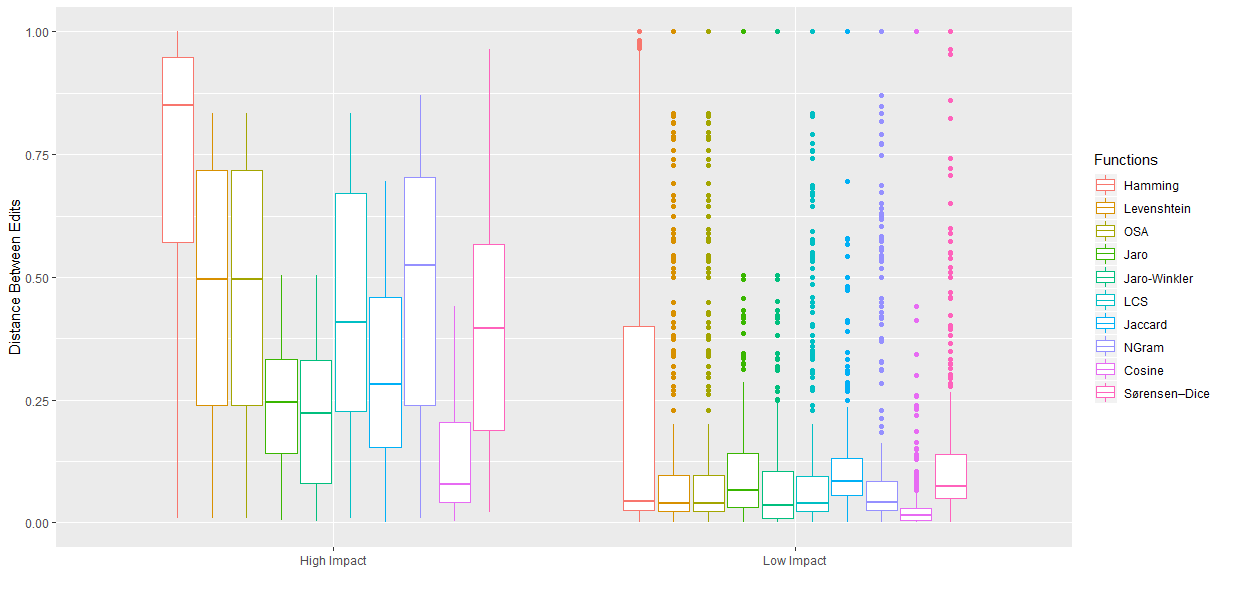
\includegraphics[height=2.3in,width=3.3in]{figs/Boxplot_SAFF_BZT.png}
% \caption{Box-plot for the distance values.}
% \label{fig:bp_dist}
% \end{figure}

\begin{figure}[h]
\centering
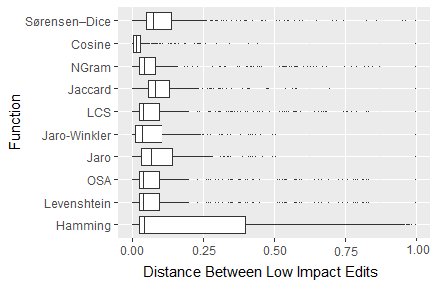
\includegraphics[height=2.3in,width=3.3in]{figs/Boxplot_SAFF_BZT_LOW2.png}
\caption{Box-plot for low impact distance values.}
\label{fig:bp_dist_l}
\end{figure}

\begin{figure}[h]
\centering
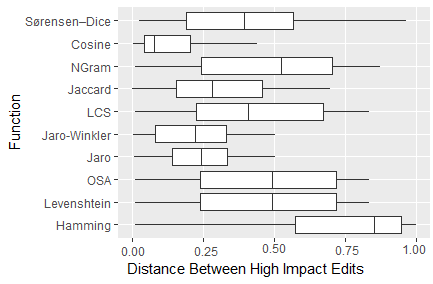
\includegraphics[height=2.3in,width=3.3in]{figs/Boxplot_SAFF_BZT_HIGH2.png}
\caption{Box-plot for high impact distance values.}
\label{fig:bp_dist_h}
\end{figure}

As for automatic classification, we need to define an effective \textit{impact threshold}, for each distance function, we run an exploratory study to find the optimal configuration for using each function. By impact threshold, we mean the distance value for classifying an edit as low or high impact. For instance, consider a defined impact threshold of x\% to be used with function \textit{f}. When analyzing an edit from a specification document, if \textit{f} provides a value lower than \textit{x}, we say the edit is \textit{low impact}, otherwise it is \textit{high impact}. Therefore, we design a study where, for each function, we vary the defined \textit{impact threshold} and we observed how it would impact Precision and Recall. Our goal with this analysis is to identify the more effective configuration for each function. We range the impact threshold between $[0;1]$. 

To find this optimal configuration, we consider the interception point between the Precision and Recall curves, since it reflects a scenario with less mistaken classifications (false positives and false negatives). %Figure 6 presents this analysis for all functions, except Jaccard, while Figure 5 presents the analysis for Jaccard and highlights its best configuration (impact threshold of 0.33).
Figure \ref{fig:best_jaccard} presents the analysis for the Jaccard functions. Its optimal configuration is highlighted (impact threshold of 0.33) --  the green line refers to the Precision curve, the blue line to the Recall curve, and the red circle shows the point both curves meet. Figure \ref{fig:all} presents the analysis for the other functions. 


\begin{figure}[h!] 
\centering 
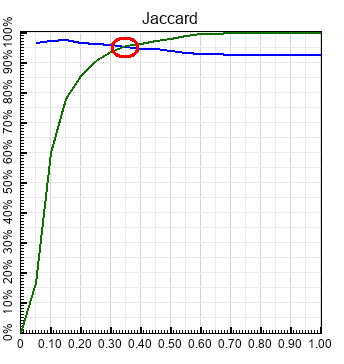
\includegraphics[width=.5\textwidth]{figs/best_Jaccard.png}
\caption{Best impact threshold for the Jaccard function.}
\label{fig:best_jaccard}
\end{figure}


\begin{figure*}[h!] 
\centering 
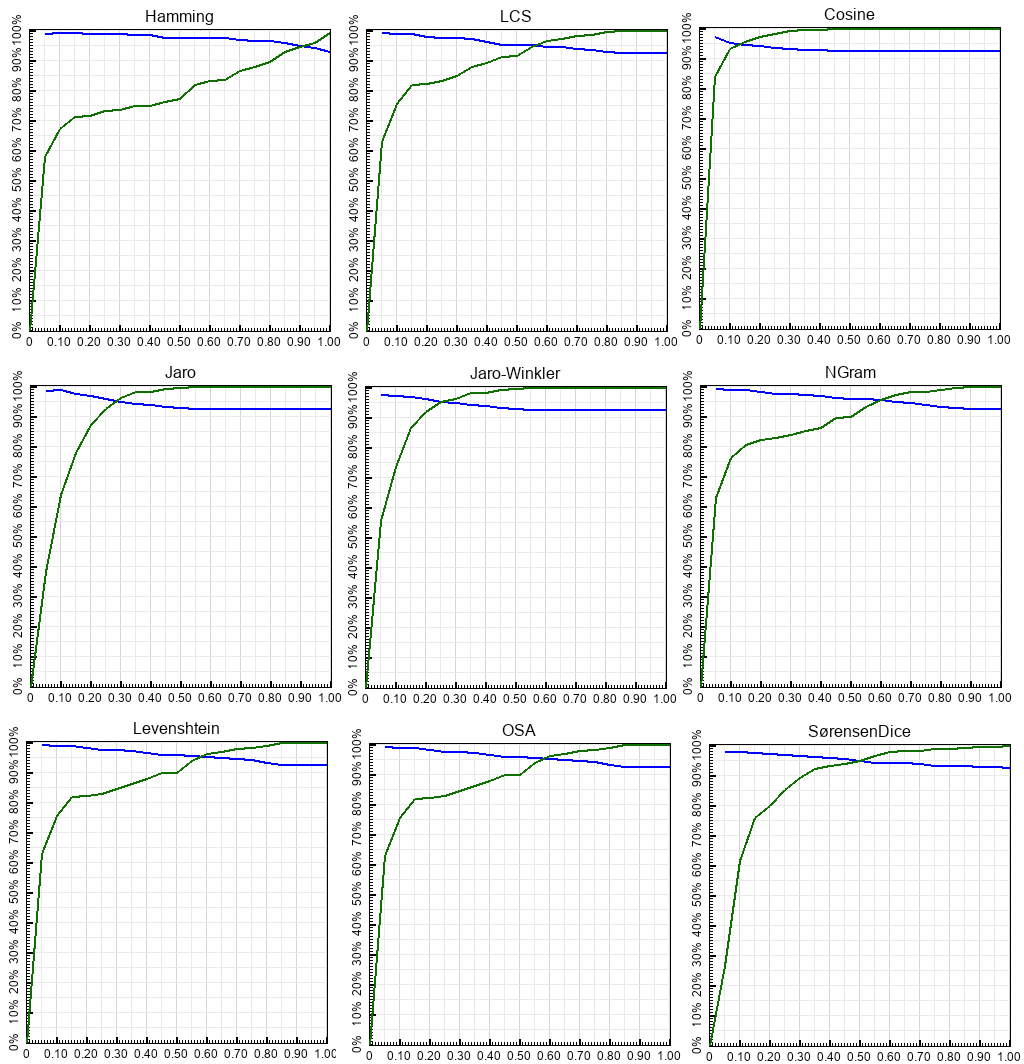
\includegraphics[width=1.0\textwidth]{figs/all.png}
\caption{Exploratory study for precision and recall per distance function.}
\label{fig:all}
\end{figure*}


Table \ref{tab:bestval} presents the optimal configuration for each function and the respective precision, recall, and accuracy values. These results reinforce our evidence to answer RQ4 since all functions presented accuracy values greater than 90\%. Moreover, we can partially answer RQ5, since now we found, considering our dataset, the best configuration for each distance function. To complement our analysis, we went to investigate which function performed the best. First, we run proportion tests considering both the functions all at once and pair-to-pair. Our results show, with 95\% of confidence, could not find any statistical differences among the functions. This means that distance function for automatic classification of edits impact is effective, regardless of the chosen function (RQ5). Therefore, in practice, one can decide which function to use based on convenience aspects (e.g., easier to implement, faster). 

\\
\\
\noindent
\vspace{2mm} %5mm vertical space
\fbox{\begin{minipage}{23em}
\textbf{RQ5: Which distance function presents the best results for classifying edits in use case documents?}
Statistically, all ten distance functions performed similarly when classifying edits from use case documents.
\end{minipage}}

\begin{table}[h]
\caption{Best configuration for each function and respective precision, recall and accuracy values.}
\resizebox{\columnwidth}{!}{%
\begin{tabular}{lcccc}
\multicolumn{1}{c}{\textbf{Function}} & \textbf{\begin{tabular}[c]{@{}c@{}}Impact \\ Threshold\end{tabular}} & \textbf{Precision} & \textbf{Recall} & \textbf{Accuracy} \\
Hamming                               & 0.91                                                                 & 94.59\%            & 94.79\%         & 90.15\%           \\
Levenshtein                           & 0.59                                                                 & 95.22\%            & 95.42\%         & 91.31\%           \\
OSA                                   & 0.59                                                                 & 95.22\%            & 95.42\%         & 91.31\%           \\
Jaro                                  & 0.28                                                                 & 95.01\%            & 95.21\%         & 90.93\%           \\
Jaro-Winkler                          & 0.25                                                                 & 95.21\%            & 95.21\%         & 91.12\%           \\
LCS                                   & 0.55                                                                 & 94.99\%            & 94.79\%         & 90.54\%           \\
Jaccard                               & 0.33                                                                 & 95.22\%            & 95.42\%         & 91.31\%           \\
NGram                                 & 0.58                                                                 & 95.41\%            & 95.21\%         & 91.31\%           \\
Cosine                                & 0.13                                                                 & 95\%               & 95\%            & 90.73\%           \\
Sørensen–Dice                         & 0.47                                                                 & 94.99\%            & 94.79\%         & 90.54\%          
\end{tabular}
}
\label{tab:bestval}
\end{table}

\section{Case Study}
\label{sec:case}
To reassure the conclusions presented in the previous section, and to provide a more general analysis, we ran new studies considering a different object, TCOM. TCOM is an industrial software also developed in the context of our cooperation with the Ingenico Brasil Ltda. It controls the execution and manages testing results of a series of hardware parts. It is important to highlight that a different team ran this project, but in a similar environment:  CLARET use cases for specification and generated MBT suites. The team also reported similar problems concerning volatile requirements, and frequent test case discards.

First, similar to the procedure applied in Section \ref{sec:procedure}, we mined TCOM's repository and collected all versions of its use case documents and their edits. Table \ref{tab:useCasesEvaluation} summarizes the collected data from TCOM. Then, we manually classified all edits between low and high impact to serve as validation for the automatic classification. Finally, we ran all distance functions considering the optimal \textit{impact thresholds} (Table \ref{tab:bestval} - second column) and calculated Precision, Recall and Accuracy for each configuration (Table \ref{tab:bestvalEvaluation}).

\begin{table}[]
\centering
\caption{Summary of the artifacts for the TCOM system.}
\label{tab:useCasesEvaluation}
\begin{tabular}{|l|l|l|l|}
\hline
     & \#Use Cases & \#Versions &\#Edits \\ \hline
TCOM &     7      &      32    &     133         \\  \hline
\end{tabular}
\end{table}



\begin{table}[h]
\caption{TCom - Evaluating the use of the found impact threshold for each function and respective precision, recall and accuracy values.}
\resizebox{\columnwidth}{!}{%
\begin{tabular}{lcccc}
\multicolumn{1}{c}{\textbf{Function}} & \textbf{\begin{tabular}[c]{@{}c@{}}Impact \\ Threshold\end{tabular}} & \textbf{Precision} & \textbf{Recall} & \textbf{Accuracy} \\
Hamming                               & 0.91                                                                 & 87.59\%            & 94\%         & 84.96\%           \\
Levenshtein                           & 0.59                                                                 & 87.85\%            & 94\%         & 85.71\%           \\
OSA                                   & 0.59                                                                 & 87.85\%            & 94\%         & 85.71\%           \\
Jaro                                  & 0.28                                                                 & 89.52\%            & 94.00\%         & 87.22\%           \\
Jaro-Winkler                          & 0.25                                                                 & 94.00\%            & 89.52\%         & 87.22\%           \\
LCS                                   & 0.55                                                                 & 89.62\%            & 95\%         & 87.97\%           \\
Jaccard                               & 0.33                                                                 & 89.52\%            & 94\%         & 87.22\%           \\
NGram                                 & 0.58                                                                 & 87.85\%            & 94\%         & 85.71\%           \\
Cosine                                & 0.13                                                                 & 88.68\%               & 94\%            & 86.47\%           \\
Sørensen–Dice                         & 0.47                                                                 & 88.68\%            & 94\%         & 86.47\%          
\end{tabular}
}
\label{tab:bestvalEvaluation}
\end{table}

As we can see, the found impact thresholds presented high precision, recall, and accuracy values when used in a different system and context (all above 84\%). This result gives as evidence that, distance functions are effective for automatic classification of edits (RQ4) and that the found impact thresholds performed well for a different experimental object (RQ5).

In a second moment,  
%Believing that the automatic classification is efficient,
we used this case study to evaluate how our approach (using distance functions for automatic classification) can help reducing test discards:
\begin{itemize}
\item \textbf{RQ6}: Can distance function be used for reducing the discard of MBT tests? 
\end{itemize}

To answer RQ6, we considered TCOM's MBT test cases generated from its CLARET files. Since all distance functions behave similarly (Section \ref{sec:res}), in this case study we used only Levenshtein's function to automatically classify the edits and to check the impact of those edits in the tests. In a common scenario, which we want to avoid, any test case that contains an updated step would be discarded. Therefore, in the context of our study, we used the following strategy \textit{``only test cases that contain high impact edits should be discarded, while test cases with low impact edits are likely to be reused with no or little updating''}. The rationale behind this decision is that low impact edits often imply on little to no changes to the system behavior. Considering system-level black-box test suites (as the ones from the projects used in our study), those tests should be easily reused. We used this strategy and we first applied Oliveira's et al.'s  classification \citep{de2016full} that divided TCOM's tests among three sets:  \textit{obsolete} -- test cases that include impacted steps; \textit{reusable} -- test cases that were not impacted by the edits; and \textit{new} -- test cases that include new steps. 

A total of 1477 MBT test cases were collected from TCOM's, where 333 were found \textit{new} (23\%), 724 \textit{obsolete} (49\%), and 420 \textit{reusable} (28\%). This data reinforces \citet{Silva:2018:SIM:3266003.3266009}'s 
conclusions showing that, in an agile context, most of an MBT test suite became obsolete quite fast. 

In a common scenario, all ``obsolete'' test cases (49\%) would be discarded throughout the development cycles. To cope with this problem, we ran our automatic analysis and we reclassified the 724 obsolete test cases among \textit{low impacted} -- test cases that include unchanged steps and updated steps classified by our strategy as "low impact"; \textit{highly impacted} -- test cases that include unchanged steps and ``high impact'' steps; and \textit{mixed}, test cases that include at least one ``high impact'' step and at least one ``low impact'' step. 


From this analysis, 109 test cases were \textit{low impacted}. Although this number seems low (15\%), those test cases would be wrongly discarded when in fact they could be easily turned into reusable. For instance, Table \ref{tab:li_tc} shows a simplified version of a ``low impacted'' test case from TCOM. As we can see, only step 2 was updated to better phrase a system response. This was an update for improving specification readability, but it does not have any impact on the system's behavior. We believe that  \textit{low impacted} test cases could be easily reused with little or no effort. In our case study, most of them need small updating that could be easily done in a single updating round, or even during test case execution. For the tester point of view, this kind of update may not be urgent and should not lead to a test case discard.

\begin{table}[]
\centering
\caption{Example of a low impacted test case.}
\begin{tabular}{|l|l|}
\hline
\begin{tabular}[c]{@{}l@{}}...\\ step 1: operator 
presses \\the terminal approving \\button.\\
step 2: system goes \\back to the terminal\\ profiling screen.\\ ...\end{tabular} & \begin{tabular}[c]{@{}l@{}}...\\ step 1: operator 
presses \\the terminal approving \\button.\\
step 2: system redirects \\the terminal to its\\ profiling screen.\\ ...\end{tabular} \\ \hline
\end{tabular}
\label{tab:li_tc}
\end{table}


The remaining test cases were classified as follows: 196 ``highly impacted'' (27\%), and 419 ``mixed'' (58\%). Table \ref{tab:hi_tc} and \ref{tab:hi_mx} show examples of highly impacted and mixed tests, respectively. In Table \ref{tab:hi_tc}, we can see that steps 3, 4, and 9 were drastically changed, which infer to a test case that requires much effort to turn it into reusable. On the other hand, in the test in Table \ref{tab:hi_mx}, we have both an edit for fixing a typo (step 2) and an edit with a requirement change (step 7). 

\begin{table}[]
\centering
\caption{Example of a highly impacted test case.}
\begin{tabular}{|l|l|}
\hline
\begin{tabular}[c]{@{}l@{}}...\\ step 3: operator presses\\  camera icon. \\ step 4: system redirects\\  to photo capture screen.\\ ...\\ step 9: operator takes a\\  picture and presses \\ the Back button.\\ ...\end{tabular} & \begin{tabular}[c]{@{}l@{}}...\\ step 3: operator selects\\ a testing plan.\\ step 4: system redirects \\ to the screen that shows\\  the selected tests.\\ ...\\ step 9: operator sets a \\ score and press Ok.\\ ...\end{tabular} \\ \hline
\end{tabular}
\label{tab:hi_tc}
\end{table}


\begin{table}[]
\centering
\caption{Example of a mixed test case.}
\begin{tabular}{|l|l|}
\hline
\begin{tabular}[c]{@{}l@{}}...\\ step 2: operator presses \\ button CANCEL to mark\\ there is no occurrence \\ description.\\ ...\\ step 7: operator presses \\ the button SEND.\\ ...\end{tabular} & \begin{tabular}[c]{@{}l@{}}...\\ step 2: operator presses \\the button CANCEL to\\
mark there is no \\occurrence description.\\ ...\\ step 7: operator takes a \\ picture of the hardware.\\ ...\end{tabular} \\ \hline
\end{tabular}
\label{tab:hi_mx}
\end{table}

To check whether our classification was in fact effective we present its confusion matrix (Table \ref{tab:conf_mat}). In general, our classification was 66\% effective (Precision). A smaller precision was expected, when compared to the precision classification from Section \ref{sec:es}, since here we consider all edits that might affect a test case, while in Section \ref{sec:es} we analyzed and classified each edit individually. However, we can see, our classification was highly effective for \textit{low impacted} test cases, and most mistaken classification relates to \textit{mixed} one (tests that combine low and high impact edits). Those were, in fact, test cases that were affected in a great deal by different types of use case editions.

% \begin{table}[]
% \caption{Confusion Matrix.}
% \begin{tabular}{c|c|c|c|c}
% %\hline
%                                                       & \multicolumn{4}{c}{Predicted} \\ %\hline
%                                                       & Low   & High   & Mixed  &      \\ \hline
% \begin{tabular}[c]{@{}c@{}}Actual\\ Low\end{tabular}   & 69    & 4      & 21     & 94   \\ \hline
% \begin{tabular}[c]{@{}c@{}}Actual\\ High\end{tabular}  & 3     & 37     & 27     & 67   \\ \hline
% \begin{tabular}[c]{@{}c@{}}Actual\\ Mixed\end{tabular} & 37    & 155    & 371    & 563  \\ \hline
%                                                       & 109   & 196    & 419    & 724  \\% \hline
% \end{tabular}
% \label{tab:conf_mat}
% \end{table}

\begin{table}[]
\centering
\caption{Confusion Matrix.}
\begin{tabular}{c|c|c|c|c}
%\hline
                                                       & \multicolumn{4}{c}{Predicted} \\ %\hline
                                                       & Low   & High   & Mixed  &      \\ \hline
\begin{tabular}[c]{@{}c@{}}Actual\\ Low\end{tabular}   & 69    & 3      & 37     & 109   \\ \hline
\begin{tabular}[c]{@{}c@{}}Actual\\ High\end{tabular}  & 4     & 37     & 155     & 196  \\ \hline
\begin{tabular}[c]{@{}c@{}}Actual\\ Mixed\end{tabular} & 21    & 27    & 371    & 419  \\ \hline
                                                       & 94   & 67    & 563    & 724  \\% \hline
\end{tabular}
\label{tab:conf_mat}
\end{table}


% functions
%         LP    HP    MP    
% LA    69    3    37    109
% HA    4    37    155    196
% MA     21    27    371    419
%         94    67    563    724

% model
%       LP    HP    MP    
% LA    75    4    30    109
% HA    12    169    15    196
% MA     6    157    256    419
%       93    330    301    724

Back to our strategy, we believe that \textit{highly impacted} or \textit{mixed} classifications indicate test cases that are likely to be discarded, since they refer to tests that would require much effort to be updated, while \textit{low impacted} tests can be reused with little to no effort. Overall, our strategy correctly classified the test cases in 66\% of the cases (Precision). Regarding \textit{low impacted} tests, we correctly classified 63\% of them. Therefore, from the 724 ``obsolete'' test cases, our strategy automatically inferred that 9.53\% of them should not be discarded.
%Therefore, in our data set, 15\% (94/724) of the first ``obsolete'' set should ideally be reclassified as reusable. Our strategy was able to automatically identify 73\% of those, which refers to the recovery from discarding of a rate of 9.53\%. 
We believe this rate can get higher when we better analyze the \textit{mixed} set. A mixed test combines low and high impact edits. However, when we manually analyzed those cases, we found several examples where, although \textit{high impact} edits were found, most test case impacts were related to \textit{low impact} edits. For instance, there was a test case composed of 104 execution steps where only one of those steps needed revision due to a \textit{high impact} use case edit, while the number of \textit{low impact} edits was seven. In a practical scenario, although we still classify it as a \textit{mixed} test case, we would say the impact of the edits was still quite small, which may indicate a manageable revision effort. Thus, we state that mixed tests need better analysis before discarding. The same approach may also work for \textit{highly impacted} tests when related to a low number of edits.

Finally, we can answer RQ6 by saying that an automatic classification using distance functions can, in fact, reduce the number of discarded test cases by at least 9.53\%. However, this rate tends to be higher when we consider \textit{mixed} tests.
\\
\\
\noindent
\vspace{2mm} %5mm vertical space
\fbox{\begin{minipage}{23em}
\textbf{RQ6: Can distance function be used for reducing the discard of MBT tests?}
The use of distance functions can reduce the number of discarded test cases by at least 9.53\%.
\end{minipage}}









\section{Threats to Validity}
\label{sec:threats}
Most of the threats for validity to the drew conclusions refer to the number of projects, use cases and test cases used in our experimental studies. Those numbers were limited to the artifacts created in the context of the selected projects. Therefore, our results cannot be generalized beyond the three projects (SAFF, BZC, and TCOM). However, it is important to highlight that all used artifacts are from real industrial systems from different contexts. 

As for conclusion validity, our studies deal with
a limited dataset. Again, since we chose to work with real, instead of artificial artifacts, the data available for analysis were limited. However, all used data were validated by the team engineers
and by the authors.

Regarding internal validity, we collected the changed set from the project's repositories, and we manually classify each change according to its impact. This manual validation was performed by at least two of the authors and, when needed, the project’s members were consulted. Moreover, we reused open-source implementations of the distance functions\footnote{https://github.com/luozhouyang/python-string-similarity}. These implementations were also validated by the first author.

\section{Related Work}
\label{sec:related}
Güldali and Mlynarski \cite{katara2006making} discuss how MBT can support agile development. For that, they emphasize the need for automation aiming that MBT artifacts can be manageable and with little effort to apply. 

Silva et al. \cite{Silva:2018:SIM:3266003.3266009} gave the first steps on investigating issues related to MBT in the context of agile development. They ran an empirical study on the evolution of specification models and their impact on generated MBT suites and found that 86\% of a test suite is often impacted, however, more than half those tests were impacted due to syntactic model edits (low impact). Those findings greatly motivated this current research. Based on them, here we propose the use of distance functions for automatically classify the test cases that are little impacted and could be reused.

Oliveira Neto et al. \cite{de2016full} discuss a series of problems related to keeping MBT suites updated during software evolution. To cope with this problem, they propose a test selection approach that uses test case similarity as input when collecting test cases that focus on recently applied changes. Oliveira Neto et al.'s approach refer as obsolete all test cases that are impacted in any way by an edit in the requirement model. However, as our study found, a great part of those tests can be little impacted, and could be easily reused, avoiding the discard of testing artifacts. 

The test case discard problem is not restricted to CLARET artifacts. Other similar cases are discussed in the literature (e.g.,\cite{de2016full,nogueira2007model}). Moreover, this problem is even greater with MBT test cases derived from artifacts that use non-controlled language \cite{pinto2012understanding}.

Other works also deal with test case evolution (e.g.,\cite{mirzaaghaei2011automatic,pinto2012understanding}). They discuss the problem and/or propose strategies for updating the testing code. Those strategies do not apply to our context, since we work with MBT test suite evolution generated from use case models. 


The use of distance functions in the context of software engineering is not new. Several works have used distance functions in different scenarios (e.g., \cite{runkler2000automatic,okuda1976method,lubis2018combination}). For instance, Runkler and Bezdek \cite{runkler2000automatic} use the Levenshtein function for automatically extract keywords from documents. In the context of MBT, Coutinho et al. \cite{coutinho2016analysis} investigated the effectiveness of a series of distance functions when used combined with strategies for suite reduction based on similarity. Although in a different context, their results go according to ours where all distance functions performed in a similar way.







\section{Concluding Remarks}
\label{sec:conclud}
In this paper, we describe a series of empirical studies ran on industrial systems intending to evaluate the use of distance functions for automatically classify the impact of edits in use case files. Our results showed that distance functions are effective to identify low impact editions. 

We also found that low impact editions often refer to test cases that can be easily updated without any effort. We believe those results can help testers to better work with MBT artifacts in the context of software evolution and avoid the discard of test cases.

%As future work we plan to expand our study with a broader set of systems; to develop a tool that, using distance functions, can help tester to identify and update low impact test cases; and investigate the use of different approaches (e.g., machine learning) to help testers to ways update highly impacted test cases and reuse history data of obsolete MBT test cases.
As future work, we plan to expand our study with a broader set of systems. We also consider developing a tool that, using distance functions, can help testers to identify and update low impact test cases. Finally, we plan to investigate the use of different approaches (e.g., machine learning) to help testers when updating highly impacted test cases and reuse history data of obsolete MBT test cases.

\begin{acks}
This research was partially supported by a cooperation between
UFCG and two companies Viceri Solution LTDA
and Ingenico do Brasil LTDA, the latter stimulated by the
Brazilian Informatics Law n. 8.248, 1991. Second and fourth authors are supported by National Council for Scientific and Technological Development
(CNPq)/Brazil (processes 429250/2018-5 and 315057/2018-1). First and third authors were supported by UFCG/CNPq and CAPES, respectively.
\end{acks}


\bibliographystyle{ACM-Reference-Format}
\bibliography{artigo}


\end{document}
